\begin{figure}[tbp]
\centering
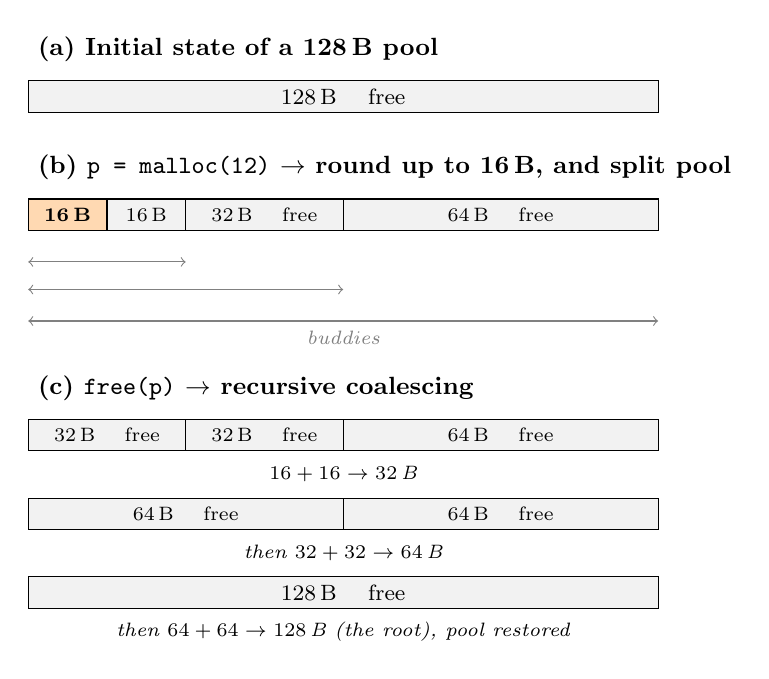
\begin{tikzpicture}[every node/.style={font=\footnotesize}]

%% Row (a): one free block, 128 B
\node[anchor=west, font=\small\bfseries] at (0.0, 7.00) {(a) Initial state of a 128\,B pool};
\draw[fill=gray!10] (0.0,6.20) rectangle (8.0,6.60);
\node at (4.0, 6.40) {128\,B \quad free};

%% Row (b): after two splits: [16 alloc'd][16 free][32 free][64 free]
\node[anchor=west, font=\small\bfseries] at (0.0, 5.50) {(b) \texttt{p = malloc(12)} $\to$ round up to 16\,B, and split pool};

\draw[fill=orange!30] (0.0,4.70) rectangle (1.0,5.10);
\node[font=\scriptsize] at (0.5, 4.90) {\textbf{16\,B}};

\draw[fill=gray!10]   (1.0,4.70) rectangle (2.0,5.10);
\node[font=\scriptsize] at (1.5, 4.90) {16\,B};

\draw[fill=gray!10]   (2.0,4.70) rectangle (4.0,5.10);
\node[font=\scriptsize] at (3.0, 4.90) {32\,B \quad free};

\draw[fill=gray!10]   (4.0,4.70) rectangle (8.0,5.10);
\node[font=\scriptsize] at (6.0, 4.90) {64\,B \quad free};

%% buddy pair annotations: three nested spans (16/16, 32/32, 64/64), labelled once on the outermost
\draw[<->, gray, thin] (0.0,4.30) -- (2.0,4.30);
\draw[<->, gray, thin] (0.0,3.95) -- (4.0,3.95);
\draw[<->, gray, thin] (0.0,3.55) -- (8.0,3.55)
  node[midway, below, font=\scriptsize\itshape] {buddies};

%% Row (c): free(p) -- a single call, recursive cascade shown one merge at a time
\node[anchor=west, font=\small\bfseries] at (0.0, 2.70)
  {(c) \texttt{free(p)} $\to$ recursive coalescing};

\draw[fill=gray!10] (0.0,1.90) rectangle (2.0,2.30);
\node[font=\scriptsize] at (1.0, 2.10) {32\,B \quad free};

\draw[fill=gray!10] (2.0,1.90) rectangle (4.0,2.30);
\node[font=\scriptsize] at (3.0, 2.10) {32\,B \quad free};

\draw[fill=gray!10] (4.0,1.90) rectangle (8.0,2.30);
\node[font=\scriptsize] at (6.0, 2.10) {64\,B \quad free};

\node[font=\scriptsize\itshape] at (4.0, 1.60) {$16+16\to32\,$B};

\draw[fill=gray!10] (0.0,0.90) rectangle (4.0,1.30);
\node[font=\scriptsize] at (2.0, 1.10) {64\,B \quad free};

\draw[fill=gray!10] (4.0,0.90) rectangle (8.0,1.30);
\node[font=\scriptsize] at (6.0, 1.10) {64\,B \quad free};

\node[font=\scriptsize\itshape] at (4.0, 0.60) {then $32+32\to64\,$B};

\draw[fill=gray!10] (0.0,-0.10) rectangle (8.0,0.30);
\node at (4.0, 0.10) {128\,B \quad free};

\node[font=\scriptsize\itshape] at (4.0, -0.40) {then $64+64\to128\,$B (the root), pool restored};

\end{tikzpicture}
\caption{A buddy allocator serving one 12-byte request from a 128-byte
  pool. (a) The pool starts as one free block. (b) The request is rounded up
  to 16\,B, and the pool is halved until a 16\,B block exists. Each split
  leaves a free \emph{buddy} of the same size next to the block it came
  from. (c) Freeing the block merges it with its buddy, and the result with
  its own buddy, until the pool is one block again. Rounding up wastes part
  of a block (here 4 of 16 bytes), but finding a block's buddy takes a
  single bit operation.}
\label{fig:buddy-alloc}
\end{figure}
